\section{Non-Uniform Sampling}
\begin{frame}{Part A}
\Large \center{\color{blue}{ Non-Uniform Sampling Algorithms}}
\end{frame}

\begin{frame}{Problem}
\begin{block}{Empirical Risk Minimization}
\center{$\min_{\wv\in\R^n} f(\wv)$}
\end{block}
\begin{equation}
    \label{eq:primalObjective}
    f(\wv):= \ell(\wv)+\lambda r(\wv)
\end{equation}
where 
\begin{equation}\label{eq:someEquationName}
    \ell(\wv) := \frac1n \sum_{i=1}^n \ell(\langle \xv_i, \wv \rangle, y_i).
\end{equation}
and 
\begin{equation}
    r(\wv) := \frac12 \|\wv\|_2^2
\end{equation}
Here, $\ell(.,y_i):\R\rightarrow\R$ is a loss function and $r(.)$ takes the role of a regularizer. 
\end{frame}

\begin{frame}{Notations}
\begin{itemize}
\item $\xv_i$: feature vector of sample $i$
\item $y_i$: label of sample $i$
\item $p_i$: probability that sample $i$ will be selected with $\sum_{j=1}^n p_j=1$
\item $\wv$: solution of objective function
\item $\eta$: stepsize for updating $\wv$
\item $\chiv_i$: subgradient of sample $i$
\item $\gv_i$: weighted subgradient of sample $i$ with $\gv_i = \frac{\chiv_i}{n p_i}$ and $\E[\gv(\wv)] = \nabla f(\wv)$
\end{itemize}
\end{frame}
\begin{frame}{NonUnifSGD}
\begin{algorithm}[H]
    \label{alg:SGD}
    \caption{Non-Uniform Stochastic Gradient Discent}
    \SetKwInput{Init}{Initialize}
    \SetKwFor{Forloop}{for}{}{end}
    \SetAlgoLined
    \KwIn{$\lambda > 0$, $p_i = \frac{\|\xv_i\|}{\sum_{j=1}^n \|\xv_j\|}, \forall i\in \{1,\ldots,n\}.$
    }
    \KwData{$\{(\xv_i,y_i)\}_{i=1}^n$.}
    \Init{
        $\wv^{1}= \textbf{0}$.
    }
    \Forloop{ $t = 1,2, \dots ,T$}{
        Sample $i_t$ from $\{1,\ldots,n\}$ based on $\p$; \\
        Set stepsize $\eta_t \leftarrow \frac{1}{\lambda t}$; \\
        Set $\chiv_{i_t}^t(\wv^{t}) \leftarrow \ell'(\langle \wv^{t}, \xv_{i_t}\rangle, y_{i_t}) \xv_{i_t}+ \lambda \nabla r(\wv^t)$;\\
        Set $\gv_{i_t}^t \leftarrow \frac{\chiv_{i_t}^t(\wv^{t})}{np_{i_t}}$;\\
        {\color{red} Set $\wv^{t+1} \leftarrow \wv^{t}-\eta_t\gv_{i_t}^t$;}
    }
    \KwOut{$\wv^{T+1}$}
\end{algorithm}
\end{frame}

%\begin{frame}{Key inequality}
%Taking the expectation over the random sampling at each step, we have the following bound:
%\begin{align*}\label{neq:fworigin}
%     \E[f(\wv^{t})]-f(\wv^*)   &\le  \frac{\eta_t}{2}\E[\|\gv_{i_t}^t\|^2]  \\
%    &+\frac{1-\lambda \eta_t}{2\eta_t} \E[\|\wv^{t}-\wv^*\|^2] - \frac{1}{2\eta_t}  \E[\|\wv^{t+1} - \wv^*\|^2]
%\end{align*}
%\end{frame}

\begin{frame}{Convergence Theorem}
\begin{theorem}
\label{theorem:basicSGD}
 Suppose $f$ is a $\lambda$-strongly convex function. If we choose the stepsize $\eta_t = \frac{1}{\lambda t }$, then after $T$ iterations of NonUnifSGD (Algorithm \ref{alg:SGD}) starting with $\wv^{1}=\bm{0}$, it holds that
    \[
        \E\big[ f\!\left(\frac1T\sum_{t=1}^T \wv^{t} \right) \big] - f(\wv^*) \le \frac{1}{2\lambda T}\sum_{t=1}^T \frac{\E[\|\gv_{i_t}^t\|^2]}{t}
    \]
    where $\gv_{i_t}^t=\frac{\chiv_{i_t}^t(\wv^{t})}{np_{i_t}}$ and the expectation is taken with respect to the distribution $\p$.
\end{theorem}
\end{frame}

%\begin{frame}{Proof Snapshot}
%\begin{figure}[H]
%        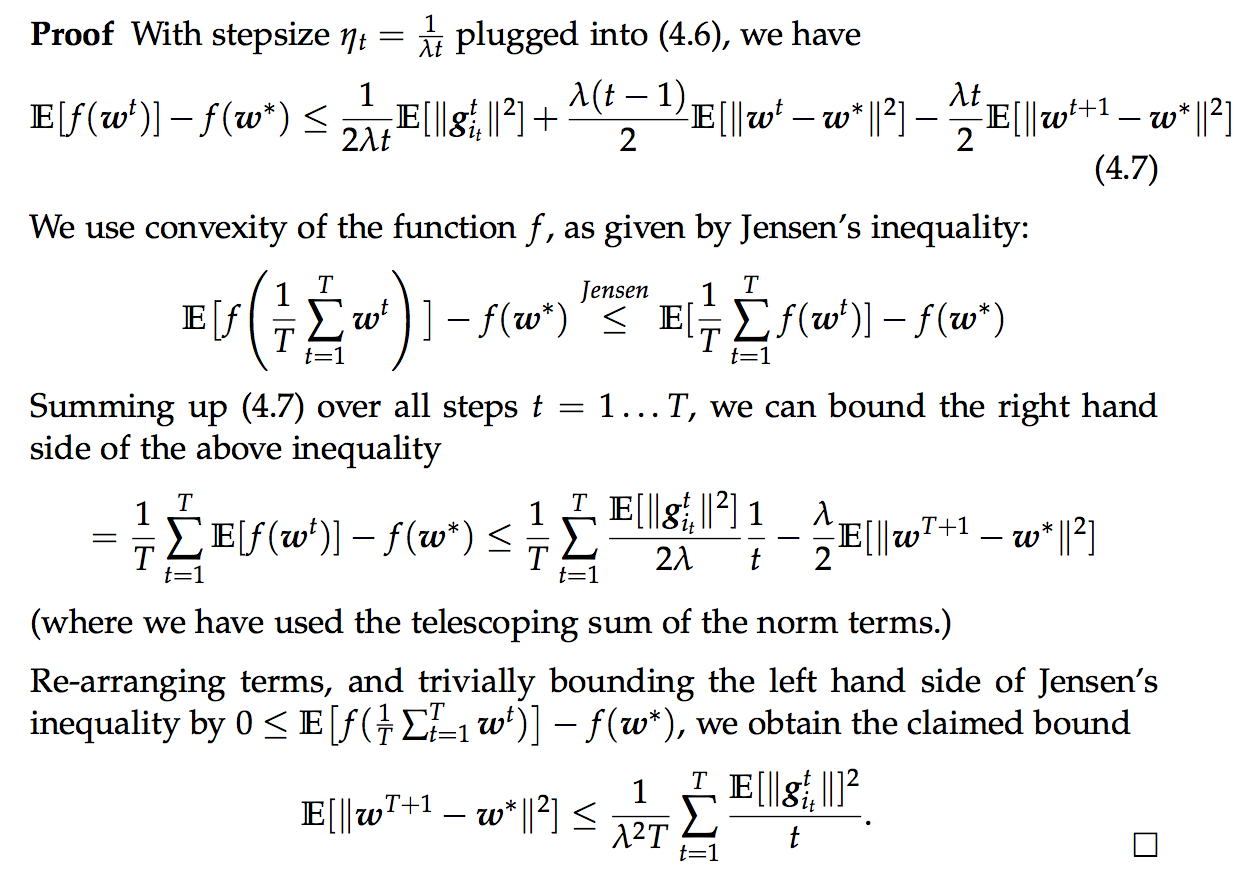
\includegraphics[width = 0.8\textwidth]{images/snapshot.png} 
%    \label{fig:two_updates}
%\end{figure}
%\end{frame}

\begin{frame}{Two corollaries}
\begin{definition}\label{def:WG}
Define $G := \max_{i, t}\{ \|\chiv_{i}^t(\wv^{t})\|^2\}$ ($i = 1\dots n$, $t=1\dots T$). \\
Define $W := \max_{i,t}\{\E[\|\chiv_{i}^t(\wv^{t})\|^2]\}$ ($i = 1\dots n$, $t=1\dots T$).
\end{definition}
\begin{corollary}\label{corollary:maxsubgrad}
Assume that $\max_{t}\{\|\chiv_{i_t}^t(\wv^t)\|^2\} \le G$ or $\E[\|\chiv_{i_t}^t(\wv^t)\|^2] \le W$ for all $t$ and $p_i > \epsilon$ for all $i=\{1\dots, n\}$,
    \begin{align*}
        \E\big[f\!\left(\frac1T\sum_{t=1}^T \wv^{t} \right)\big]- f(\wv^*) \le \frac{1}{2\lambda T} \sum_{t=1}^T \frac{G}{\epsilon nt}
\le \frac{G(\ln T+1)}{2\lambda \epsilon nT} \text{or}\\ 
        \E\big[f\!\left(\frac1T\sum_{t=1}^T \wv^{t} \right)\big]- f(\wv^*)  \le \frac{1}{2\lambda T}\sum_{t=1}^T \frac{W}{n^2\epsilon^2 t}
\le \frac{W(\ln T+1)}{2\lambda Tn^2\epsilon^2}
    \end{align*}
\end{corollary}
\end{frame}

\begin{frame}{Another Theorem for SGD}
\begin{theorem}\label{theorem:weightedSGD}
    Suppose $f$ is a $\lambda$-strongly convex function. If we choose the stepsize $\eta_t=\frac{2}{\lambda (t+1)}$, then after $T$ iterations of NonUnifSGD (Algorithm \ref{alg:SGD}) with starting point $\wv^{1}=\bm{0}$, it holds that the weighted average of the iterates satisfies
    \[
        \E\big[f(\frac{2}{T(T+1)}\sum_{t=1}^{T}t \wv^{t})\big] - f(\wv^*) \le 
        \frac{2}{\lambda(T+1)} \max_{t} \E[\|\gv_{i_t}^t\|^2]
    \]
    where $\gv_{i_t}^t=\frac{\chiv_{i_t}^t(\wv^{t})}{np_{i_t}}$,
    and the expectation is taken with respect to the distribution $\p$.
\end{theorem}
\end{frame}

\begin{frame}{Dual Problem}
\begin{block}{Dual Objective Function}
\begin{equation*}\label{eq:dual}
\max_{\alphav\in \R^n} D(\alphav):=\frac1n \sum_{i=1}^n -\ell_i^*(-\alpha_i) - \lambda r^*(\vv(\alphav)).  
\end{equation*}
\end{block}
The relationship between primal variable $\wv$ and dual variable $\alphav$ is
\begin{equation*}\label{eq:wdualupdate}
    \wv(\alphav) := \nabla r^*(\vv(\alphav)), \vv(\alphav):=\frac{1}{\lambda n} \sum_{i=1}^n \alpha_i\xv_i
\end{equation*}
where $\alphav\in \R^n$.
\end{frame}

\begin{frame}{NonUnifSDCA}
\begin{algorithm}[H]
    \label{alg:SDCA}
    \caption{Non-Uniform Stochastic Dual Coordinate Ascent}
    \SetKwInput{Init}{Initialize}
    \SetKwFor{Forloop}{for}{}{end}
    \SetAlgoLined
    \KwIn{$\lambda > 0$, $p_i = \frac{\|\xv_i\|}{\sum_{j=1}^n \|\xv_j\|}$, $\forall i\in \{1,\ldots,n\}$.
    }
    \KwData{$\{(\xv_i,y_i)\}_{i=1}^n$}
    \Init{
        $\alphav^1 = \bm{0}$, $\wv^{1}= \bm{0}$.    }
    \Forloop{ $t = 1,2, \dots ,T$}{
        Sample $i_t$ from $\{1,\ldots,n\}$ based on $\p$; \\
        Calculate $\Delta \alpha_{i_t}^{t} = \argmax_{\Delta \alpha_{i_t}^t}[-\frac{\lambda n}{2}\|\wv^{t}+\frac{1}{\lambda n}\Delta \alpha_{i_t}^t \xv_{i_t} \|^2-\ell_{i_t}^*(-(\alpha_{i_t}^{t}+\Delta\alpha_{i_{t}}^t))]$; \\ 
        {\color{red} Set $\alpha_{i_{t}}^{t+1}\leftarrow \alpha_{i_{t}}^{t}+\Delta\alpha_{i_t}^{t}$};\\
        {\color{red} Set $\wv^{t+1}\leftarrow \wv^{t}+\frac{1}{\lambda n}\Delta\alpha_{i_t}^{t}\xv_{i_t} $};\\
    }
        \KwOut{$\wv^{T+1}$}
\end{algorithm}
\end{frame}
